\documentclass[12pt]{article}
\usepackage[paperwidth=24cm,paperheight=27cm,margin=0cm]{geometry}
\usepackage{fontspec}
\usepackage{xcolor}
\usepackage{tikz}
\usetikzlibrary{arrows.meta}
\pagestyle{empty}
\setlength{\parindent}{0pt}
\setmainfont{Times New Roman}

\definecolor{BrandBlue}{HTML}{005496}
\definecolor{FlowGreen}{HTML}{2E7D32}
\definecolor{FlowOrange}{HTML}{B26A00}
\definecolor{FlowGray}{HTML}{4B5563}
\definecolor{LightBlue}{HTML}{EAF3FB}
\definecolor{LightGreen}{HTML}{ECF7EE}
\definecolor{LightOrange}{HTML}{FFF4E2}
\definecolor{LightGray}{HTML}{F3F4F6}
\definecolor{LineColor}{HTML}{475569}
\definecolor{BorderColor}{HTML}{94A3B8}
\definecolor{TextColor}{HTML}{1F2937}
\definecolor{MutedText}{HTML}{6B7280}
\definecolor{NoteFill}{HTML}{FFF8DB}

\newcommand{\flowstep}[5]{%
	\draw[rounded corners=6pt, fill=#3, draw=BorderColor, line width=1pt] (6.15,#1) rectangle (20.55,#1-1.80);
	\draw[rounded corners=6pt, fill=#2, draw=#2, line width=1pt] (6.15,#1) rectangle (20.55,#1-0.58);
	\fill[#2] (6.15,#1-0.44) rectangle (20.55,#1-0.58);
	\node[anchor=center, text=white, font=\bfseries\fontsize{15}{17}\selectfont] at (13.35,#1-0.30) {#4};
	\node[anchor=center, align=center, text width=13.70cm, text=TextColor, font=\fontsize{14}{16}\selectfont] at (13.35,#1-1.18) {#5};
}

\begin{document}
\noindent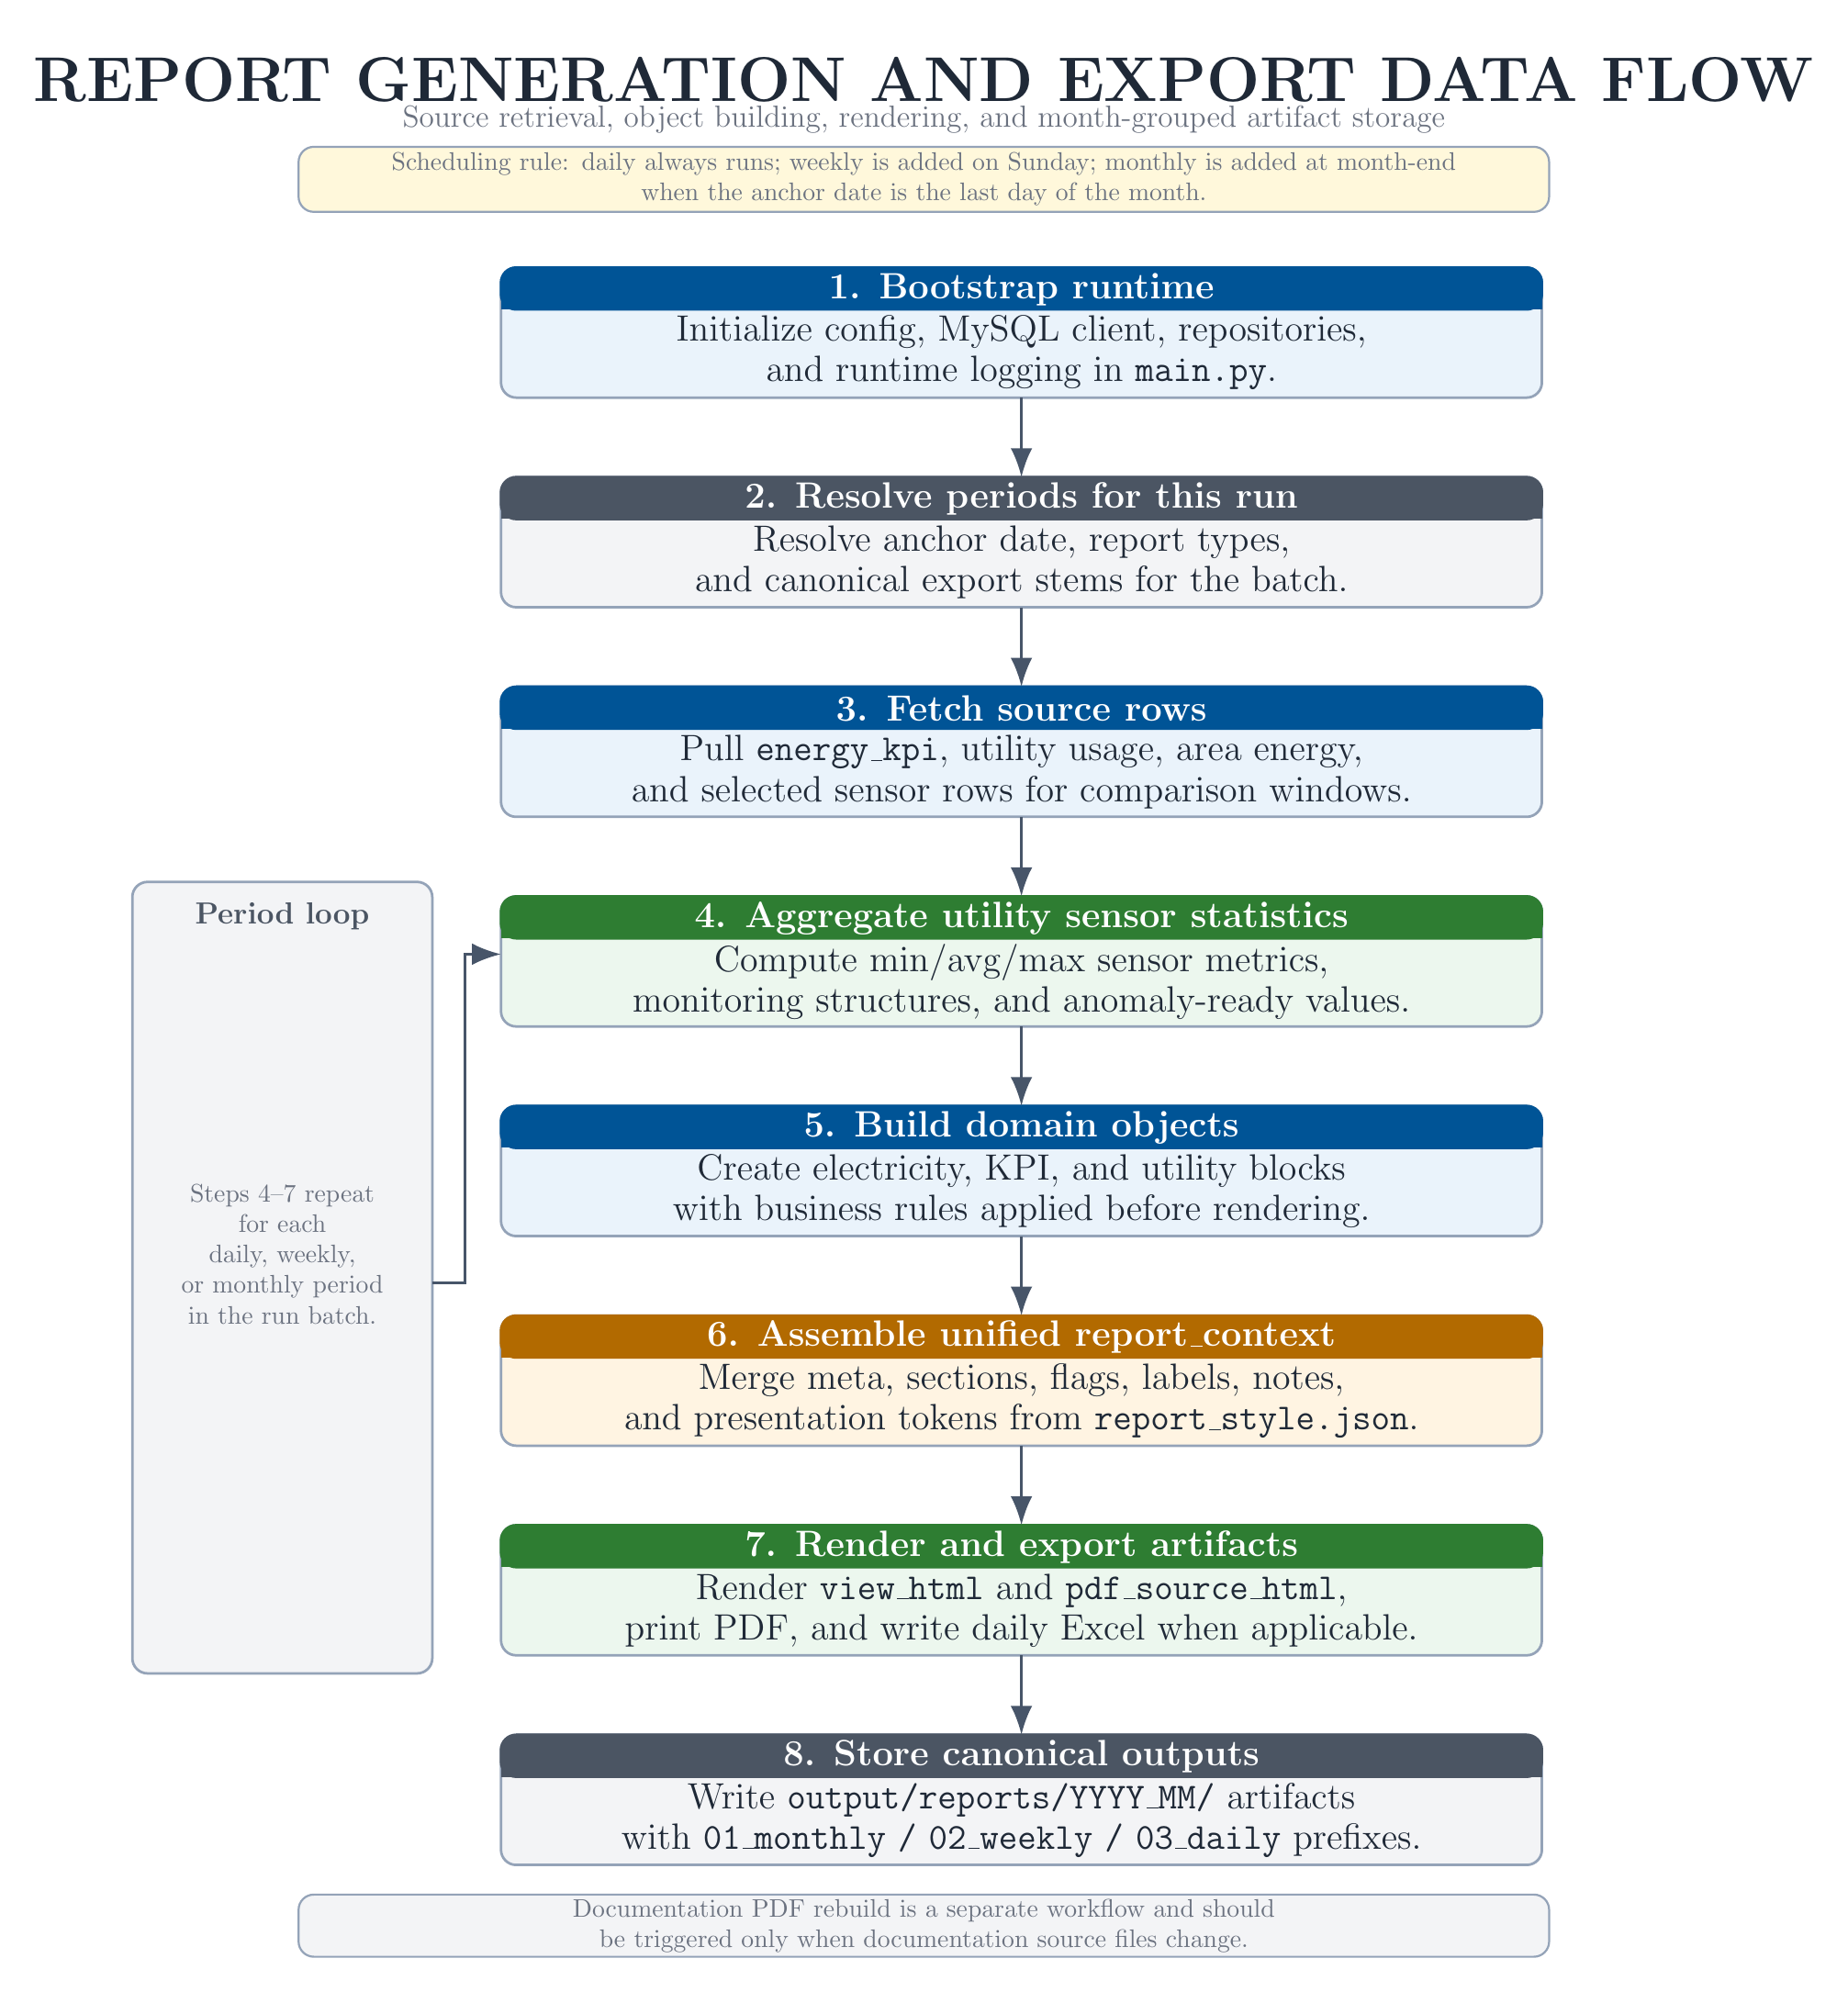
\begin{tikzpicture}[x=1cm,y=1cm]
	\fill[white] (0,0) rectangle (24,27);

	\node[font=\bfseries\fontsize{25}{28}\selectfont, text=TextColor] at (12,26.25) {REPORT GENERATION AND EXPORT DATA FLOW};
	\node[align=center, text width=15.40cm, font=\fontsize{12}{14}\selectfont, text=MutedText] at (12,25.70) {Source retrieval, object building, rendering, and month-grouped artifact storage};

	\draw[rounded corners=6pt, fill=NoteFill, draw=BorderColor, line width=0.8pt] (3.35,24.42) rectangle (20.65,25.32);
	\node[anchor=center, align=center, text width=16.30cm, text=MutedText, font=\fontsize{10}{12}\selectfont] at (12,24.87) {Scheduling rule: daily always runs; weekly is added on Sunday; monthly is added at month-end\\when the anchor date is the last day of the month.};

	\flowstep{23.65}{BrandBlue}{LightBlue}{1. Bootstrap runtime}{Initialize config, MySQL client, repositories,\\and runtime logging in \texttt{main.py}.}
	\flowstep{20.75}{FlowGray}{LightGray}{2. Resolve periods for this run}{Resolve anchor date, report types,\\and canonical export stems for the batch.}
	\flowstep{17.85}{BrandBlue}{LightBlue}{3. Fetch source rows}{Pull \texttt{energy\_kpi}, utility usage, area energy,\\and selected sensor rows for comparison windows.}
	\flowstep{14.95}{FlowGreen}{LightGreen}{4. Aggregate utility sensor statistics}{Compute min/avg/max sensor metrics,\\monitoring structures, and anomaly-ready values.}
	\flowstep{12.05}{BrandBlue}{LightBlue}{5. Build domain objects}{Create electricity, KPI, and utility blocks\\with business rules applied before rendering.}
	\flowstep{9.15}{FlowOrange}{LightOrange}{6. Assemble unified report\_context}{Merge meta, sections, flags, labels, notes,\\and presentation tokens from \texttt{report\_style.json}.}
	\flowstep{6.25}{FlowGreen}{LightGreen}{7. Render and export artifacts}{Render \texttt{view\_html} and \texttt{pdf\_source\_html},\\print PDF, and write daily Excel when applicable.}
	\flowstep{3.35}{FlowGray}{LightGray}{8. Store canonical outputs}{Write \texttt{output/reports/YYYY\_MM/} artifacts\\with \texttt{01\_monthly / 02\_weekly / 03\_daily} prefixes.}

	\foreach \upper/\lower in {21.85/20.75,18.95/17.85,16.05/14.95,13.15/12.05,10.25/9.15,7.35/6.25,4.45/3.35} {
		\draw[-{Latex[length=4mm,width=3mm]}, line width=1.1pt, draw=LineColor] (13.35,\upper) -- (13.35,\lower);
	}

	\draw[rounded corners=6pt, fill=LightGray, draw=BorderColor, line width=1pt] (1.05,15.15) rectangle (5.20,4.20);
	\node[anchor=center, align=center, text=FlowGray, font=\bfseries\fontsize{13}{15}\selectfont] at (3.125,14.67) {Period loop};
	\node[anchor=center, align=center, text width=3.35cm, text=MutedText, font=\fontsize{10}{12}\selectfont] at (3.125,10.00) {Steps 4--7 repeat\\for each daily, weekly,\\or monthly period\\in the run batch.};
	\draw[-{Latex[length=4mm,width=3mm]}, line width=1.1pt, draw=LineColor] (5.20,9.60) -- (5.65,9.60) -- (5.65,14.15) -- (6.15,14.15);

	\draw[rounded corners=6pt, fill=LightGray, draw=BorderColor, line width=0.8pt] (3.35,0.28) rectangle (20.65,1.14);
	\node[anchor=center, align=center, text width=16.20cm, text=MutedText, font=\fontsize{10}{12}\selectfont] at (12,0.71) {Documentation PDF rebuild is a separate workflow and should be triggered only when documentation source files change.};
\end{tikzpicture}
\end{document}
